\documentclass[tikz, crop, border = {2pt 2pt 2pt 2pt}]{standalone}

\usepackage{concmath-otf}
\usetikzlibrary{calc, angles, quotes, patterns}
\usetikzlibrary{decorations.pathreplacing, decorations.pathmorphing, calligraphy}

\begin{document}
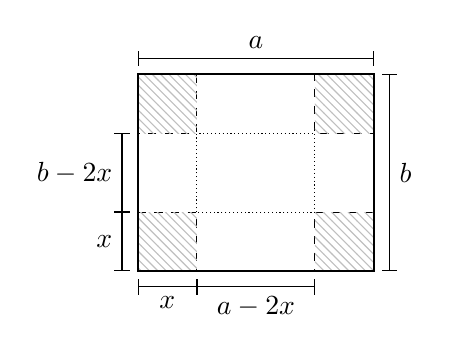
\begin{tikzpicture}
	\def\xpos{3cm}
	\def\ypos{2.5cm}
	\def\cutout{0.75cm}

	\draw[dashed] (0, \cutout) -| (\cutout, 0); 
	\fill[pattern = north west lines, pattern color = lightgray] (0, \cutout) rectangle (\cutout, 0);
	\draw[dashed] (\xpos, \cutout) -| ++ (-\cutout, -\cutout);
	\fill[pattern = north west lines, pattern color = lightgray] (\xpos, \cutout) rectangle ++ (-\cutout, -\cutout);
	\draw[dashed] (\cutout, \ypos) |- ++ (-\cutout, -\cutout);
	\fill[pattern = north west lines, pattern color = lightgray] (\cutout, \ypos) rectangle ++ (-\cutout, -\cutout);
	\draw[dashed] (\xpos, {\ypos - \cutout}) rectangle ++ (-\cutout, \cutout);
	\fill[pattern = north west lines, pattern color = lightgray] (\xpos, {\ypos - \cutout}) rectangle ++ (-\cutout, \cutout); 
	\draw[densely dotted] (\cutout, \cutout) rectangle ({\xpos - \cutout}, {\ypos - \cutout});

	\def\shiftpos{0.2cm}
	\draw[shift = {(0, -\shiftpos)}, |-|] (0, 0) -- node[below]{$x$} ++ (\cutout, 0);
	\draw[shift = {(-\shiftpos, 0)}, |-|] (0, 0) -- node[left]{$x$} ++ (0, \cutout);
	\draw[shift = {(0, \shiftpos)}, |-|] (0, \ypos) -- node[above]{$a$} ++ (\xpos, 0); 
	\draw[shift = {(\shiftpos, 0)}, |-|] (\xpos, 0) -- node[right]{$b$} ++ (0, \ypos);

	\draw[shift = {(0, -\shiftpos)}, |-|] (\cutout, 0) -- node[below]{$a - 2x$} ++ ({\xpos - 2*\cutout}, 0);
	\draw[shift = {(-\shiftpos, 0)}, |-|] (0, \cutout) -- node[left]{$b - 2x$} ++ (0, {\ypos - 2*\cutout});

	\draw[thick] (0, 0) rectangle (\xpos, \ypos);
\end{tikzpicture}
\end{document}
